\section{臨界、原子炉と核データ}

\subsection{増倍率と臨界}
核分裂連鎖反応では、核分裂の反応数が指数関数的に増減する。
1つの中性子が核分裂を引き起こし、2つの中性子が放出される体系を考える。この2つの核分裂中性子がどちらも
次の核分裂を起こす場合、この体系の中性子増倍率$k$は次のようになる。
\begin{equation}
  k = \frac{\text{発生した核分裂中性子のうち核分裂を起こす数}}{\text{核分裂を起こした中性子数}} = \frac{2}{1} = 2
\end{equation}
実際には核分裂反応はバラバラなタイミングで起こるが、簡単のために「世代」という概念を導入して考える。
丁度アニメーションのフレームと同じで、バラバラなタイミングで起こる核分裂反応を、あるタイミングで一気に
発生するものとして考える。1フレームあたりの時間は、核分裂が発生してから次の核分裂が発生するまでの平均的な
時間を使う。この時間を\emph{即発中性子寿命}、または\emph{世代時間}と呼ぶ。
中性子増倍率はある世代の中性子数を一つ前の世代の中性子数で割ったものとしても定義される。
\begin{equation}
  k = \frac{\text{ある世代の中性子数}}{\text{一つ前の世代の中性子数}}
\end{equation}
この中性子増倍率$k$が1より大きい状態を\emph{超臨界}、1より小さい状態を\emph{未臨界}、1の状態を\emph{臨界}と呼ぶ。
\[
k \; \left\{
  \begin{array}{ll}
    > 1 & \text{超臨界} \\
    = 1 & \text{臨界} \\
    < 1 & \text{未臨界}
  \end{array}
\right.
\]

\subsection{中性子と原子核の反応}
中性子は電荷を持たないため原子核に近づきやすく、原子核と\SI{e-12}{\centi\metre}程度まで近づくと
原子核と相互作用する。この相互作用は、大きく散乱反応(scattering)と吸収反応(absorption)に分けられる。

\subsubsection{散乱反応}
散乱反応はさらに\emph{弾性散乱}(elastic scattering)と\emph{非弾性散乱}(inelastic scattering)の2つに分けられる。
弾性散乱では中性子と原子核の運動エネルギーは保存されるため、一般には中性子の運動エネルギーの一部が原子核(ターゲット核)
に移り中性子の運動方向とエネルギーが変化する。弾性散乱には、中性子が原子核に取り込まれずに原子核のポテンシャルで散乱される
ポテンシャル散乱と、中性子が一旦原子核に取り込まれ複合核となった後にエネルギーを失わずに放出される共鳴散乱がある。
非弾性散乱ではターゲット核に移ったエネルギーの一部が原子核の励起エネルギーに使われる。
そのため、非弾性散乱は中性子のエネルギーがターゲット核の最低の励起エネルギーよりも大きい場合にのみ起こる。
\begin{figure}[htbp]
  \centering
  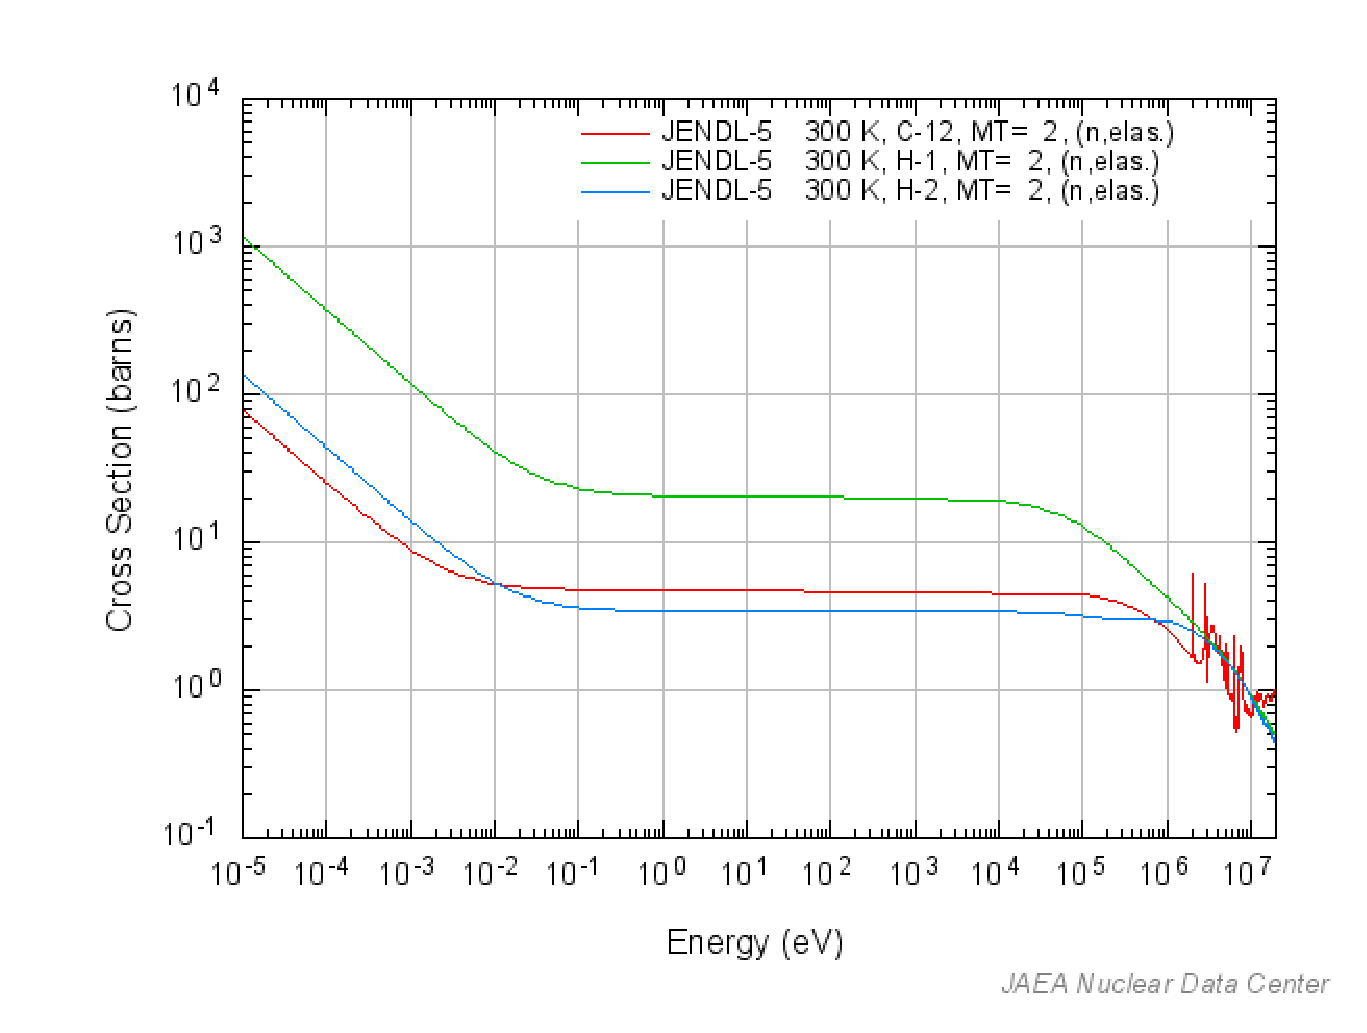
\includegraphics[width=0.8\textwidth]{figure/CrossSecElastic.eps}
  \caption{\ce{^{12}C},\ce{^{1}H},\ce{^{2}H}の弾性散乱(MT=2)の断面積}
  \label{fig:neutron_scattering}
\end{figure}

\begin{figure}[htbp]
  \centering
  \includegraphics[width=0.8\textwidth]{figure/U238Zr90Inela.eps}
  \caption{\ce{^{238}U},\ce{^{90}Zr}の非弾性散乱(MT=4)の断面積}
  \label{fig:neutron_inelastic_scattering}
\end{figure}

\begin{figure}[htbp]
  \centering
  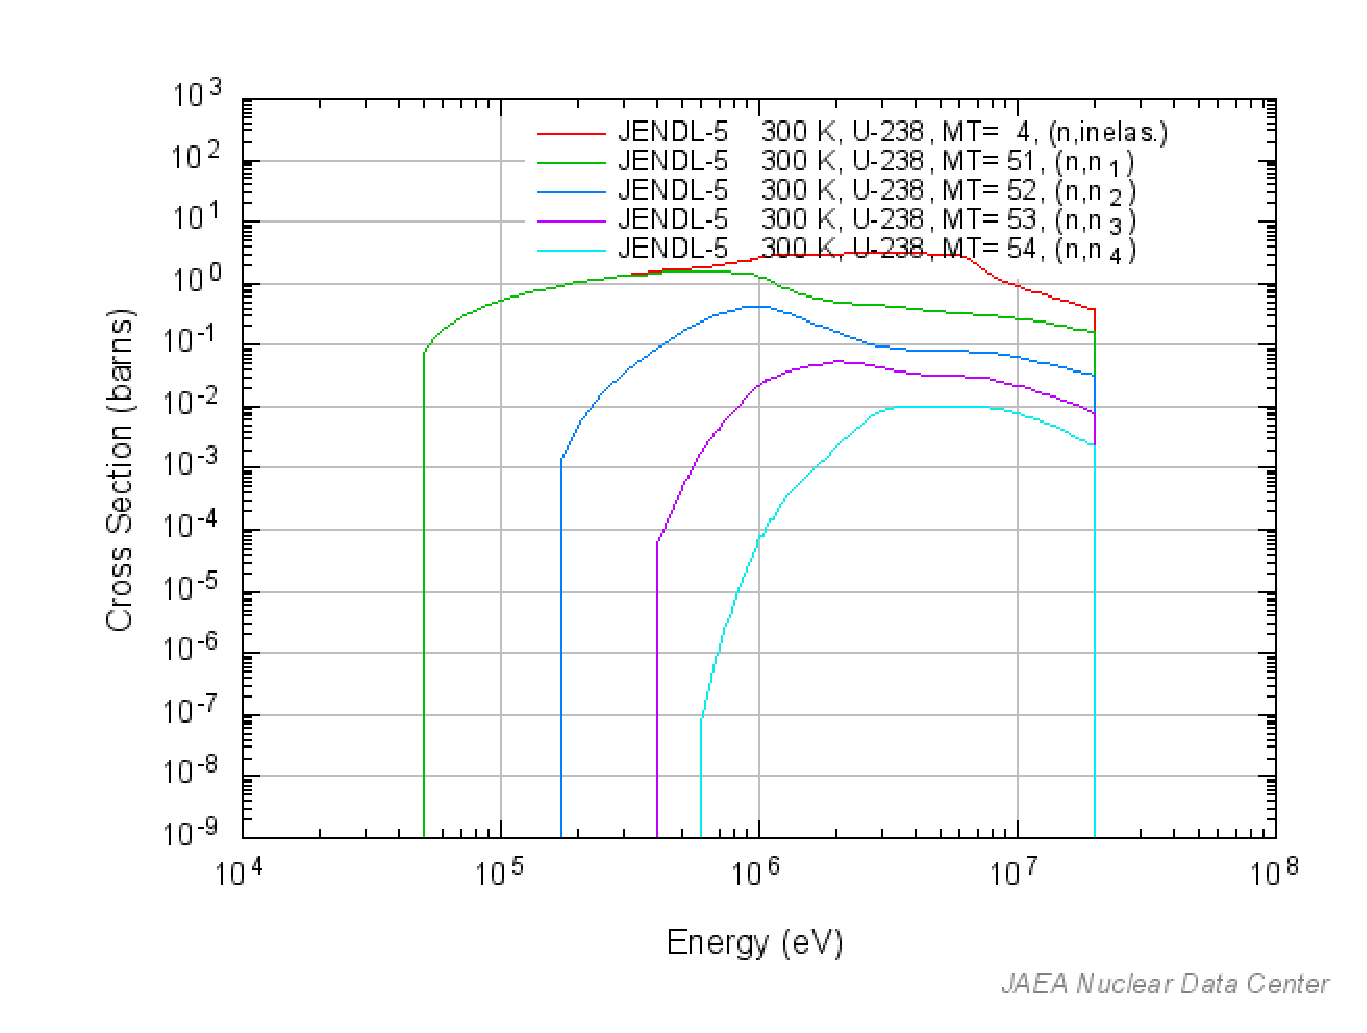
\includegraphics[width=0.8\textwidth]{figure/U238Inela_nx.eps}
  \caption{\ce{^{238}U}の非弾性散乱(MT=4,51,52,53,54)の断面積}
  \label{fig:neutron_scattering_reaction}
\end{figure}


\subsubsection{吸収反応}
原子核に中性子が取り込まれると、入射中性子のエネルギーと中性子の結合エネルギーの和の分だけ励起された複合核
が形成される。この複合核は不安定であるため、その後様々な反応を起こして安定な状態に戻ろうとする。
吸収反応この過程を経る反応の総称(散乱反応は除く)でその後の反応によってさらに多くの種類に分けられる。
これに分類されるものとしては、複合核から$\gamma$線を放出する放射捕獲反応、荷電粒子を放出する荷電粒子放出反応などがある。
原子炉において利用される核分裂反応や、入射中性子のエネルギーが高い場合に起こる2個以上の中性子が放出される反応も
この吸収反応に分類される。

\begin{figure}[htbp]
  \centering
  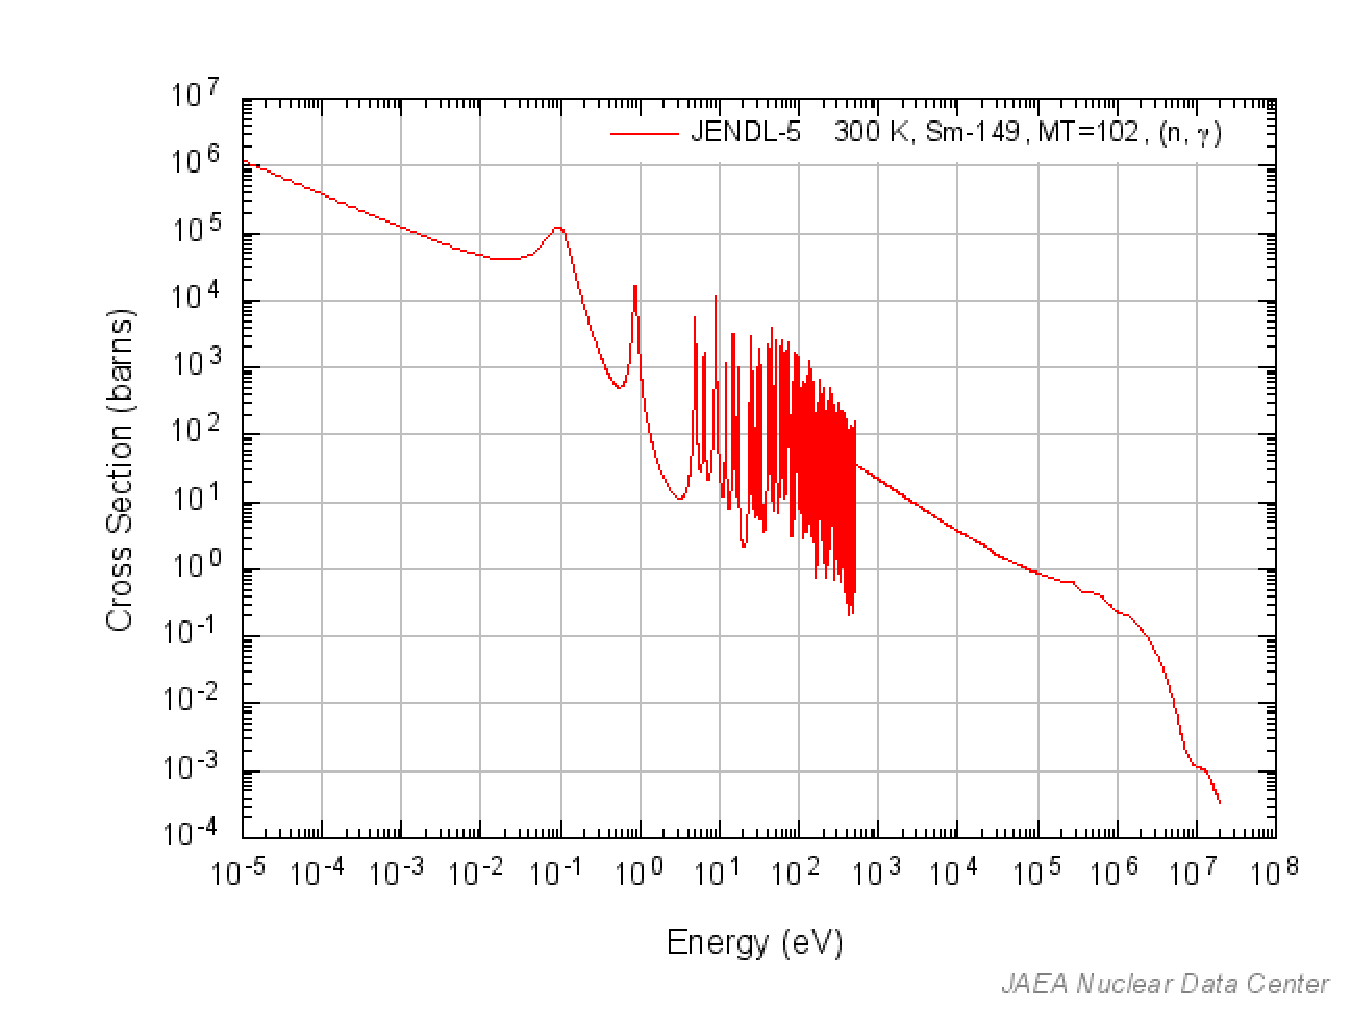
\includegraphics[width=0.8\textwidth]{figure/SmMT102.eps}
  \caption{\ce{^{149}Sm}の吸収反応(MT=102)の断面積}
  \label{fig:neutron_absorption}
\end{figure}

\begin{figure}[htbp]
  \centering
  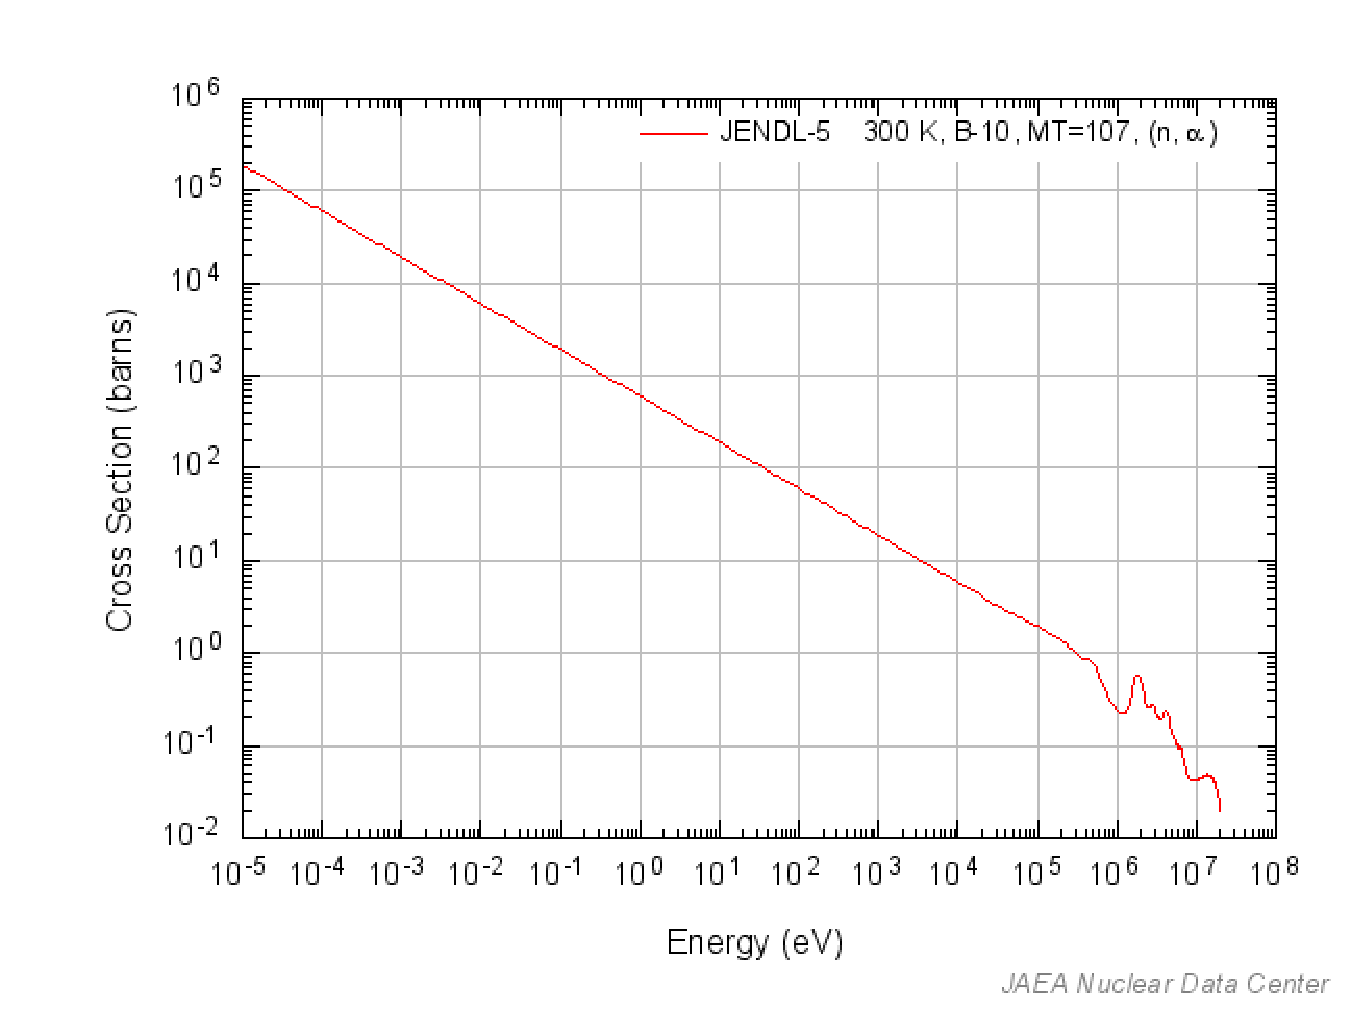
\includegraphics[width=0.8\textwidth]{figure/B10MT107.eps}
  \caption{\ce{^{10}B}の吸収反応(MT=107)の断面積}
  \label{fig:neutron_capture}
\end{figure}

\begin{figure}[htbp]
  \centering
  \includegraphics[width=0.8\textwidth]{figure/U235Fission.eps}
  \caption{\ce{^{235}U}の核分裂反応(MT=18)の断面積}
  \label{fig:neutron_fission}
\end{figure}

\begin{figure}[htbp]
  \centering
  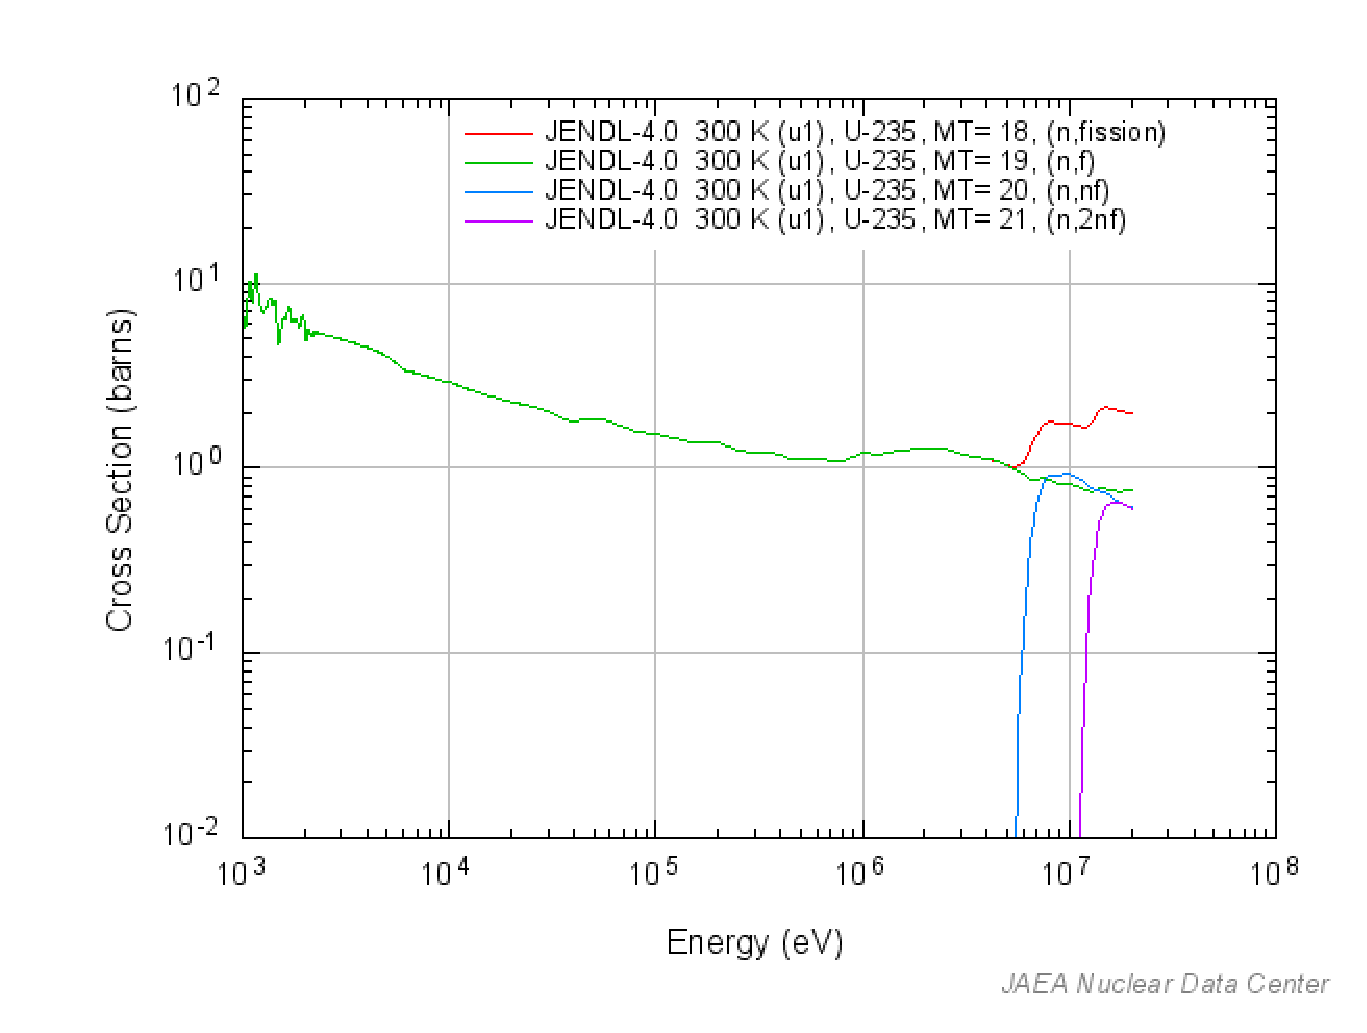
\includegraphics[width=0.8\textwidth]{figure/U235Fiss_xnf.eps}
  \caption{\ce{^{235}U}の核分裂反応(MT=18,19,20,21)の断面積}
  \label{fig:neutron_fission_U238}
\end{figure}
% 章ごとの参考文献欄
\printbibliography[segment=\therefsegment,heading=subbibliography]

\newpage
